\documentclass[../main.tex]{subfiles}
\graphicspath{{\subfix{../figures/}}}

\begin{document}
\chapter{Current Baseline} \label{chap:baseline}
This chapter unveils the mathematical model of our controlled plant, what OJ has achieved with their PI controller and other available resources they provide.

\section{Validation Environment Setup} \label{sec:env_intro}
At OJ, we test our thermostats in an enclosed chamber insulated by foam (Fig. \ref{fig:narnia}) where there are eight sensors to measure the temperature of:
\begin{enumerate}
    \item Two points inside the floor
    \item Four points at different heights of the inside air
    \item Three points of the cold air outside of the chamber
\end{enumerate}
\begin{figure}[htbp]
    \centering
    \includegraphics[width=\linewidth]{figures/narnia.png}
    \caption{OJ's facility for testing thermostats}
    \label{fig:narnia}
\end{figure}
As shown in figure \ref{fig:temp_dist}, the temperatures vary by height. Still, let us assume a perfect scenario where they are uniformly distributed within each material, allowing us to utilize only the average sensor readouts denoted as
\begin{enumerate}
    \item Floor temperature $T_f$
    \item Inside air temperature $T_a$
    \item Outside air temperature $T_{out}$
\end{enumerate}
\begin{figure}[H]
    \centering
    \begin{subfigure}{0.49\textwidth}
        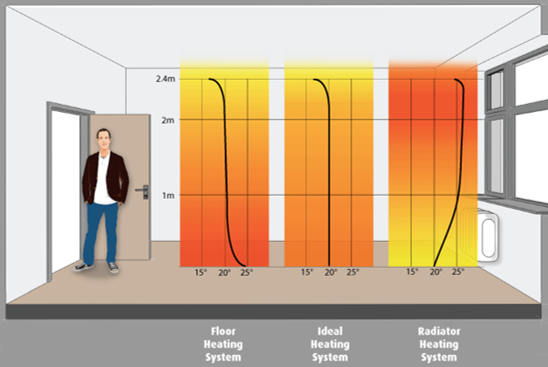
\includegraphics[width=\linewidth]{figures/temp_dist.png}
        \caption{Temperature distribution by height \cite{warmup_heat_distribution}}
        \label{fig:temp_dist}
    \end{subfigure}
    \begin{subfigure}{0.49\textwidth}
        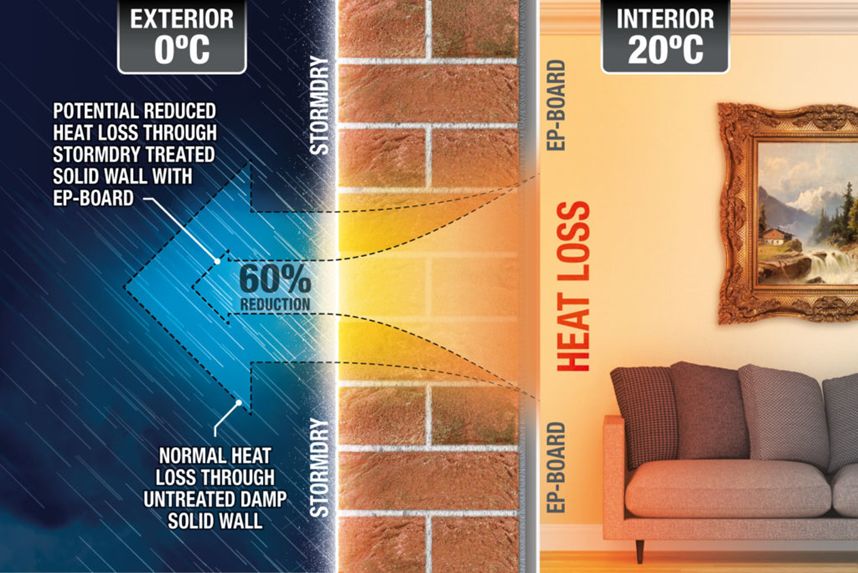
\includegraphics[width=\linewidth]{figures/conductive_loss.png}
        \caption{Heat loss through walls \cite{heatloss_thru_walls}}
        \label{fig:cond_loss}
    \end{subfigure}
    \caption{Thermodynamics of a floor-heated room}
    \label{fig:room_char}
\end{figure}

The process begins with a conduction coil warming up the concrete floor. This coil has a resistance $\Gamma = 12\,(k\Omega)$ and receives an input current $I = 2\,(A)$, hence the total power supply
\begin{align} \label{eq:psup}
    P_0 &= \Gamma I^2 \\
    &= 12 \times 2^2 = 48~(kW)  \notag
\end{align}
Current $I$ can be adjusted accordingly to different house sizes while the resistance $\Gamma = 12\,(k\Omega)$ stays constant by European standards. Then, a portion of this energy transfers to the air before exiting to the exterior coldness. Figure \ref{fig:cond_loss} illustrates this phenomenon, which is known as heat conduction. 

Our plant's actual dynamics, which include three phases, are recorded every second and visualized in figure \ref{fig:actual_dynamics}. First, the room cools down naturally from 28 (\degree C) until balancing with the air temperature. Then, it is heated from step 67,174 to reach 22.5 (\degree C) before UWG5's PI controller starts regulating from step 71,000. These plots reveal that our system has very slow dynamics, so training a data-driven controller by directly interacting with it is not feasible. Thus, we must train and evaluate our models in a simulated environment before deploying them to real hardware.
\begin{figure}
    \centering
    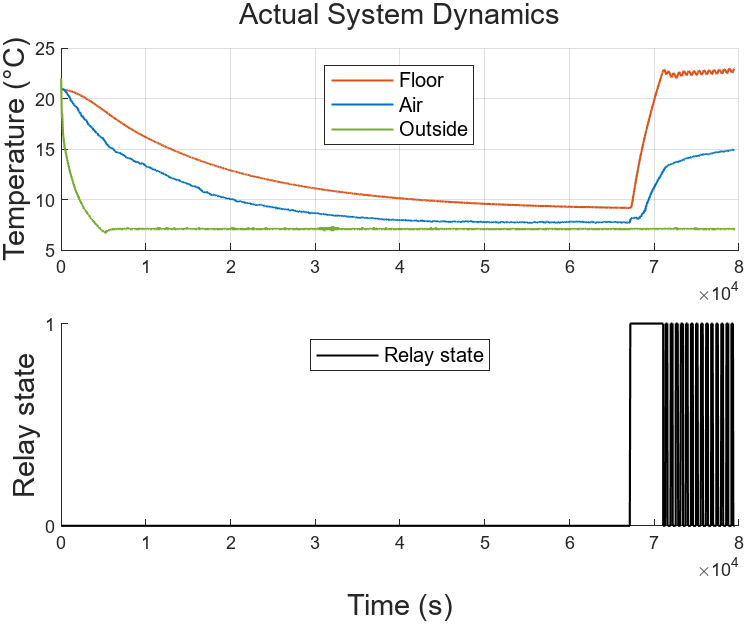
\includegraphics[width=\linewidth]{figures/ActualSystemDynamics.png}
    \caption{Actual system dynamics of OJ's testing chamber}
    \label{fig:actual_dynamics}
\end{figure}


\section{Environment Modeling with Physics} \label{sec:env_model}
The above setup is simple to derive its dynamics from physics. Indeed, if we turn on the relay for a short time $dt$, the floor temperature increases by a small amount $dT_f$ as in equation \ref{eq:floor_temp}.
\begin{align} \label{eq:floor_temp}
    m_f C_f dT_f &= (P_0 - Q_x) dt \notag \\
    \Leftrightarrow \dot{T}_f &= \frac{1}{m_f C_f}(P_0 - Q_x)
\end{align}
\begin{itemize}
    \item $T_f~(K)$: absolute floor temperature
    \item $m_f~(kg)$: total floor mass
    \item $C_f~(Jkg^{-1}K^{-1})$: heat capacity of concrete
    \item $Q_x~(J)$: heat transfer from floor to air
\end{itemize}
Consequently, the air gets hotter by $dT_a$:
\begin{align}
    m_a C_a \,dT_a &= (Q_x - Q_{loss}) \,dt \notag \\
    \Leftrightarrow \dot{T}_a &= \frac{1}{m_a C_a} (Q_x - Q_{loss})
    \label{eq:air_temp}
\end{align}
\begin{itemize}
    \item $T_a~(K)$: absolute air temperature
    \item $m_a~(kg)$: total air mass
    \item $C_a~(Jkg^{-1}K^{-1})$: heat capacity of the air
    \item $Q_{loss}~(J)$: heat loss through walls
\end{itemize}
According to Fourier's law, conducted heat $Q_x$ and $Q_{loss}$ are calculated by the following equations:
\begin{equation}
    \begin{split}
        Q_x &= -\frac{k_f A_f}{d_f}(T_a - T_f) \\
        Q_{loss} &= -\frac{k_w A_w}{d_w}(T_{out} - T_a) 
    \end{split}
    \label{eq:heat_transfer}
\end{equation}
\begin{itemize}
    \item $k_f$, $k_w~(W/mK)$: heat conductivity of concrete and foam
    \item $A_f$, $A_w~(m^2)$: total surface area of the floor and walls
    \item $d_f$, $d_w~(m)$: thickness of the floor and walls
    \item $T_{out}$: ambient temperature outside
\end{itemize}
From equations \ref{eq:floor_temp}, \ref{eq:air_temp}, \ref{eq:heat_transfer}, we have a system of ordinary differential equations (ODEs) \ref{eq:narnia_odes} and its equivalent state space \ref{eq:narnia_ss}.
\begin{equation}
    \left\{
    \begin{aligned}
        \dot{T}_f &= \frac{1}{m_f C_f}\left[P_0 +\frac{k_f A_f}{d_f}(T_a - T_f)\right] \\
        \dot{T}_a &= \frac{1}{m_a C_a}\left[-\frac{k_f A_f}{d_f}(T_a - T_f) - \frac{k_w A_w}{d_w}(T_{out} - T_a)\right]
    \end{aligned}
    \right.
    \label{eq:narnia_odes}
\end{equation}

\begin{equation}
    \begin{bmatrix}
      \dot{T}_a \\
      \dot{T}_f 
    \end{bmatrix} = \begin{bmatrix}
      -\frac{k_f A_f}{d_f m_a C_a} - \frac{k_w A_w}{d_w m_a C_a} & \frac{k_f A_f}{d_f m_a C_a} \\
      \frac{k_f A_f}{d_f m_c C_f} & -\frac{k_f A_f}{d_f m_c C_f}
    \end{bmatrix} \begin{bmatrix}
      T_a \\
      T_f
    \end{bmatrix} + \begin{bmatrix}
      0 \\
      \frac{1}{m_f C_f}
    \end{bmatrix}P_0 + \begin{bmatrix}
      \frac{k_w A_w}{d_w m_a C_a} \\
      0
    \end{bmatrix}T_{out}
    \label{eq:narnia_ss}
\end{equation}

To simplify our code, especially for future parameter estimation, let us set
\begin{equation*}
\begin{aligned}
    &u = \left\{ \begin{aligned}
        P_0 = 48 ~kW \text{ when relay is on} \\
        0 ~kW \text{ when relay is off}
    \end{aligned} \right. \\
    &\mathbf{x} = \begin{bmatrix}
      T_a \\
      T_f
    \end{bmatrix} \text{  plant's state vector} \\
    &p_1 = \frac{1}{m_f C_f};~~
    p_2 = \frac{k_f A_f}{d_f}\\
    &p_3 = \frac{1}{m_a C_a};~~
    p_4 = \frac{k_w A_w}{d_w}\\
    &\mathbf{p} = \begin{bmatrix}
        p_1 & p_2 & p_3 & p_4
    \end{bmatrix}^\top \text{  plant's parameters} \\
    &T_{out} = w(t) \text{  is a measurable disturbance}
\end{aligned}
\end{equation*}
and receive the simplified version of \ref{eq:narnia_ss}
\begin{align}\label{eq:narnia_sss}
    \dot{\mathbf{x}} &=
        \begin{bmatrix}
            -p_2 p_3 - p_3 p_4 & p_2 p_3 \\
            p_1 p_2 & -p_1 p_2
        \end{bmatrix}\mathbf{x}
        + \begin{bmatrix}
            0 \\
            p_1
        \end{bmatrix}u + \begin{bmatrix}
            p_3 p_4 \\
            0
        \end{bmatrix}w \\
    \mathbf{y} &= \begin{bmatrix}
        1 & 0 \\
        0 & 1
    \end{bmatrix}\mathbf{x} \notag
\end{align}

Table \ref{tab:init_values} presumes some initial values, with which we have the response in figure \ref{fig:hypo_dynamics}. Although this presumption does not perfectly match our data in figure \ref{fig:actual_dynamics}, the general behaviors are very similar, i.e., the floor is always hotter than air $T_f \geq T_a$, cooling them down takes a few hours, whereas heating is much more rapid. Be careful; the parameters are in hours, whereas figure \ref{fig:actual_dynamics} and \ref{fig:hypo_dynamics} display in seconds.
\begin{table}[htb]
\caption{Initial values for validation}
\label{tab:init_values}
\centering
    \begin{tabular}{|l|l|l|l|}
    \hline
    \textbf{Variable} & \textbf{Unit} & \textbf{Value} & \textbf{Description} \\ \hline
    \hline
    $m_f$ & $kg$ & 600 & total floor mass \\ \hline
    $C_f$ & $J/kgK$ & 1005 & heat capacity of concrete \\ \hline
    $d_f$ & $m$ & 0.05 & floor thickness \\ \hline
    $k_f$ & $J/mKh$ & 7200 & heat conductivity of concrete \\ \hline
    $A_f$ & $m^2$ & 5 & floor area \\ \hline
    $d_w$ & $m$ & 0.02 & wall thickness \\ \hline
    $m_a$ & $kg$ & 13.475 & air mass \\ \hline
    $C_a$ & $J/kgK$ & 1005 & heat capacity of air \\ \hline
    $k_w$ & $J/mKh$ & 126 & heat conductivity of foam \\ \hline
    $A_w$ & $m^2$ & 19.8 & total wall area \\ \hline
    $T_a(0)$ & $K$ & 293 & initial air temperature \\ \hline
    $T_f(0)$ & $K$ & 295 & initial floor temperature \\ \hline
    \end{tabular}
\end{table}
\begin{figure}
    \centering
    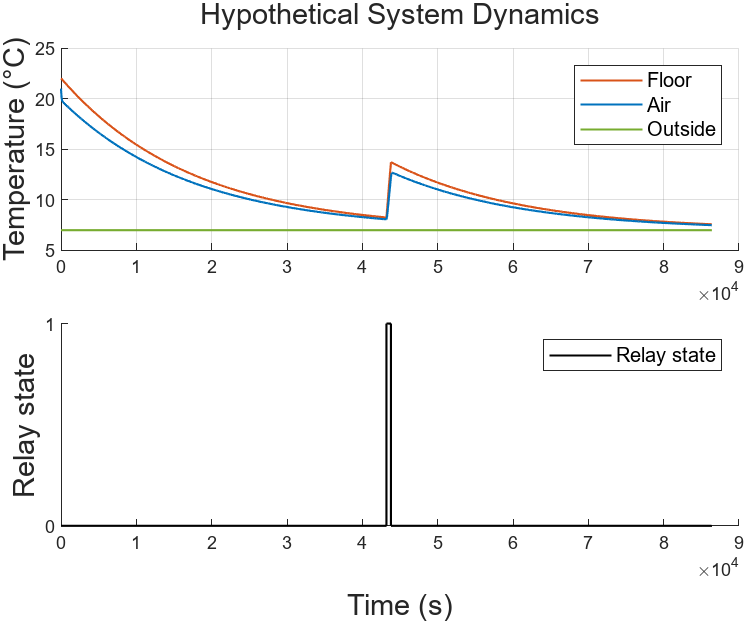
\includegraphics[width=\linewidth]{figures/HypotheticalSystemDynamics.png}
    \caption{Hypothetical system dynamics with parameters in Table \ref{tab:init_values}}
    \label{fig:hypo_dynamics}
\end{figure}

\nomenclature[D]{ODE}{ordinary differential equation}
\nomenclature[N]{$t$, $k$}{continuous and discrete time, respectively}
\nomenclature[N]{$\mathbf{A}, \mathbf{B}, \mathbf{C}, \mathbf{D}, \mathbf{E}$}{State space matrices. All bold capital characters are matrices.}
\nomenclature[N]{$\mathbf{R}, \mathbf{N}, \mathbf{N}^*$}{Set of real, integer, non-zero integers, respectively.}
\nomenclature[N]{$\mathbf{x}, \mathbf{y}$}{State and output vector in a dynamical system's state space form. All bold non-capital characters are vectors.}
\nomenclature[N]{$K$}{Kelvin, a unit of temperature, $0K = -273\degree C$}
\nomenclature[N]{$T$}{absolute temperature in Kelvin}
\nomenclature[N]{$Q$}{Heat, also known as thermal energy, measured in Joule}
\nomenclature[N]{$J$}{Joule, a unit of heat and energy}
\nomenclature[N]{$W$}{Watt, a unit of power, 1W = 1 Joule/second ($Js^{-1}$) = 3600 Joule/hour ($Jh^{-1}$)}
\nomenclature[N]{$m$}{kg, total mass of an object in kilogram. If $m$ is a unit as in $4(m)$, it means "a length of 4 meters."}
\nomenclature[N]{$V$}{$m^3$, volume of an object in cubic meters. If $V$ is a unit as in $4(V)$, it means "a voltage of 4 volts."}
\nomenclature[N]{$M$}{$kgm^{-3}$, density of a material in kilogram per cubic meter}


\section{Parameter Estimation with Data} \label{sec:env_estim}
To create a practical controller via simulation, we first need to improve our system model by estimating their precise values with actual data (Sec. \ref{sec:env_intro}). A deterministic estimator such as Least Squared Error (LSE) is perfect for this task thanks to its simplicity and explainability. Recursive Least Squares (RLS) and Weighted Least Squares (WLS) are also promising. RLS updates parameters iteratively with new data, making its memory efficiency ideal for real-time applications. WLS assigns distinct weights to data points, enhancing model accuracy in the presence of varying data reliability or outliers. However, our data has none of these issues, so a basic LSE is sufficient. To begin, equation \ref{eq:narnia_sss} must be reformed so that it can fit with multiple samples, that is
\begin{alignat}{2}
    (\ref{eq:narnia_sss}) 
    &\Leftrightarrow
    \dot{\mathbf{x}} &&= \mathbf{Ax} + \mathbf{B}u + \mathbf{E}w \notag \\ 
    &\Leftrightarrow
    \dot{\mathbf{x}}^\top &&= \begin{bmatrix}
        \mathbf{x}^\top & u & w
    \end{bmatrix}\begin{bmatrix}
        \mathbf{A}^\top \\ \mathbf{B}^\top \\ \mathbf{E}^\top
    \end{bmatrix} \notag \\
    &\Leftrightarrow
    \mathbf{Y} &&= \mathbf{X}\theta
\label{eq:narnia_lse}
\end{alignat}

These elements' sizes are:
\begin{multicols}{2}
\begin{itemize}
    \item $\mathbf{Y} \in \mathbb{R}^{m \times 2}$
    \item $\mathbf{X} \in \mathbb{R}^{m \times 4}$
    \item $\theta \in \mathbb{R}^{4 \times 2}$
    \item $m$: number of samples
\end{itemize}
\end{multicols}
To avoid hidden errors caused by the PI controller, we only utilize the first 71,000 discrete samples, i.e., only natural cooling and heating. Thus, equation \ref{eq:narnia_lse} is implemented in MATLAB using forward integrator as:
\begin{equation}
\begin{split}
    \dot{\mathbf{x}} &\leftarrow \mathbf{x}[2:71,000] \\
    \mathbf{x} &\leftarrow \mathbf{x}[1:70,999]
\end{split}
\end{equation}
Subsequently, LSE returns a unique solution in equation \ref{eq:lse}.
\begin{align} \label{eq:lse}
    &\hat{\theta} = \left(\mathbf{X}^\top\mathbf{X}\right)^{-1}\mathbf{X}^\top\mathbf{Y}\\
    \Leftrightarrow { }
    &\hat{\theta} = \begin{bmatrix}
        -7.89e-4 & 3.45e+6 \\
        6.73e-4 & -3.45e+6 \\
        0 & 4.7841 \\
        1.2e-4 & 0
    \end{bmatrix} \notag \\
    \Leftrightarrow { }
    &\mathbf{p} = \begin{bmatrix}
        4.7841 & 7.21e+5 & 9.5e-10 & 1.26e+5
    \end{bmatrix}^\top \notag
\end{align}
Figure \ref{fig:fit} shows a perfect fit between our estimate and the records, approving our understanding of the state-space in equation \ref{eq:narnia_ss}. Note that finding exact values for $\mathbf{p}$ is not strictly necessary. Yet, it is a real physical property that might be useful for future extension with various chamber sizes and features of a model-based controller.
\begin{figure}[H]
\centering
\begin{subfigure}{0.9\textwidth}
    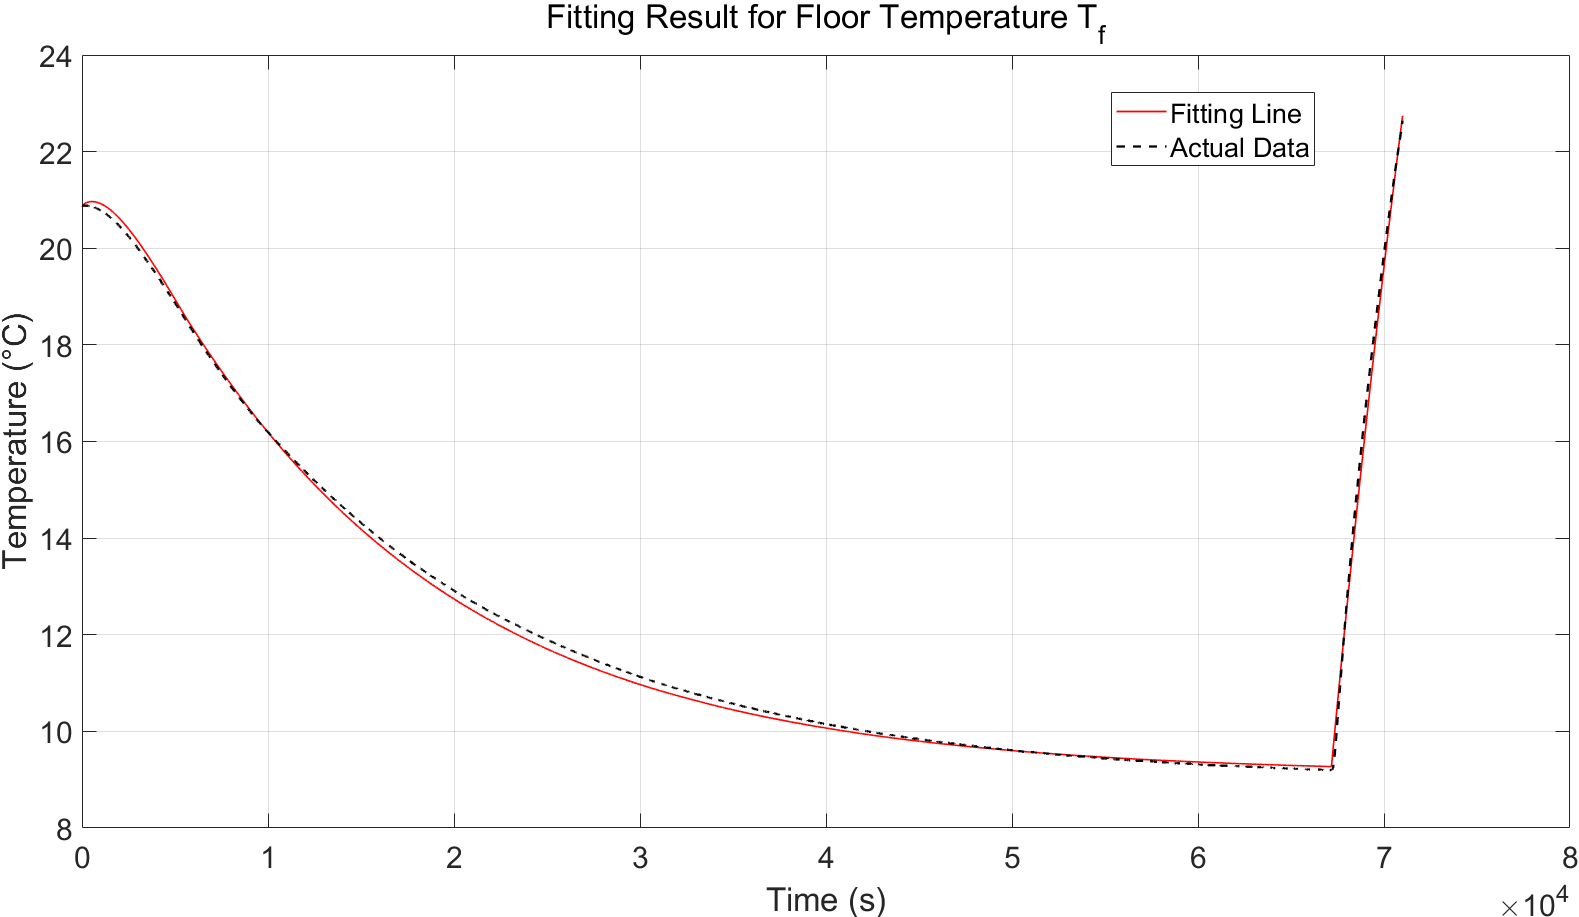
\includegraphics[width=\linewidth]{figures/fitting_floor_temp.png}
    \label{fig:fit_floor}
\end{subfigure}
\begin{subfigure}{0.9\textwidth}
    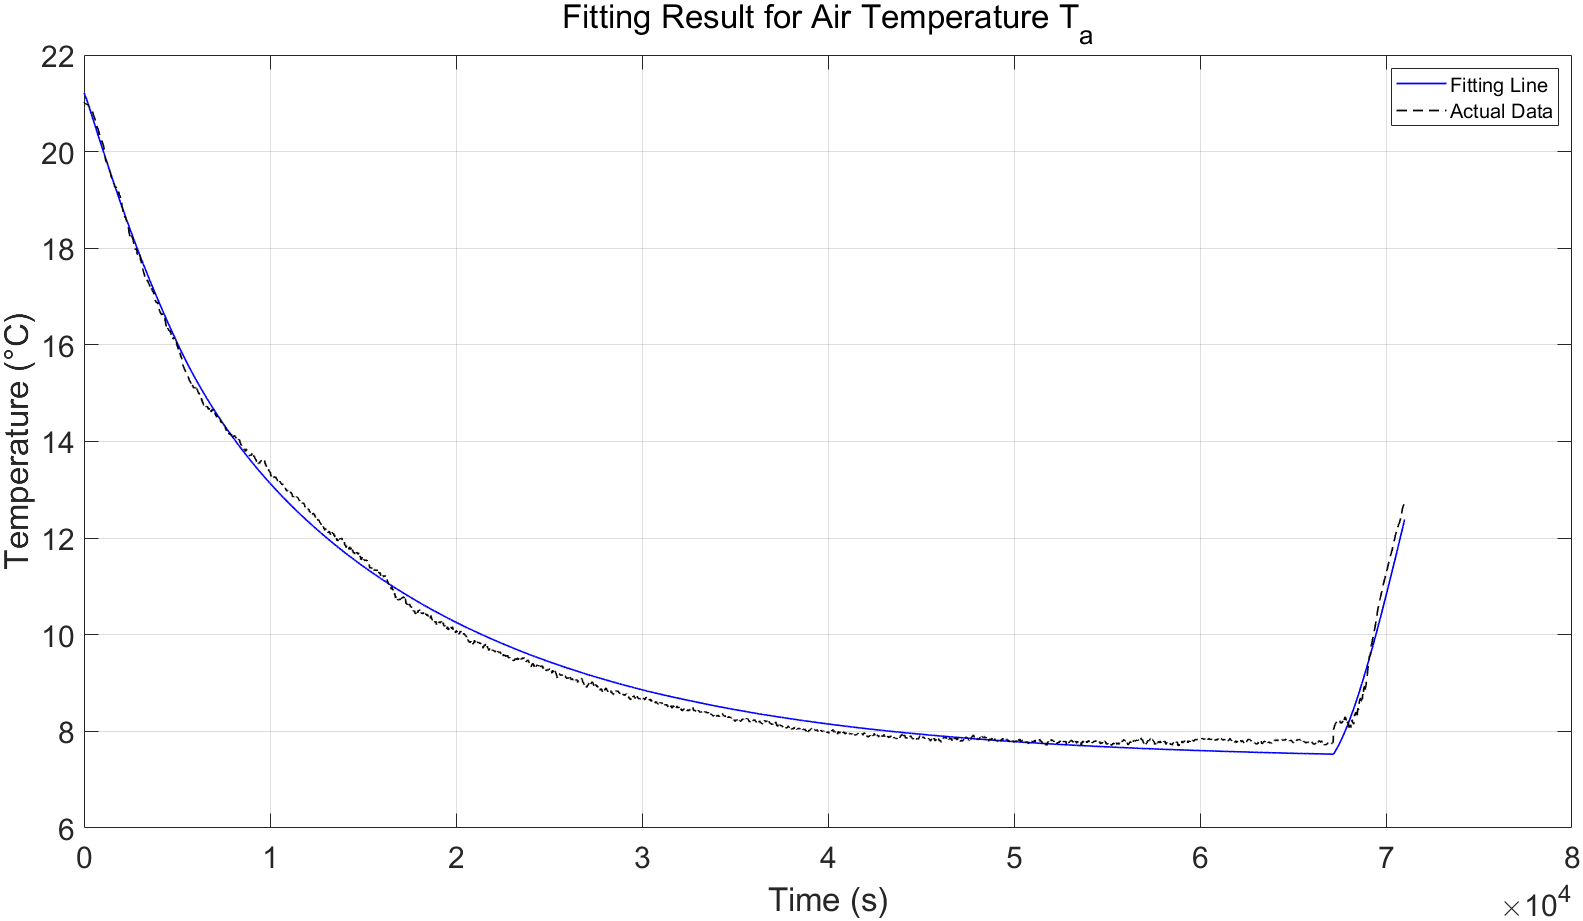
\includegraphics[width=\linewidth]{figures/fitting_air_temp.png}
    \label{fig:fit_air}
\end{subfigure}
\caption{Parameter estimation results for $T_f$ and $T_a$}
\label{fig:fit}
\end{figure}

\nomenclature[D]{System Identification}{a process of recreating the model from measured data instead of physics}

\section{Baseline of the Current Controller} \label{sec:env_baseline}
Control signals such as torque, valve position, or voltage are continuous in most autonomous applications. They are typically generated by regulating a fixed-period PWM signal from microcontrollers with a duty cycle $D \in [0,1]$. Generally, a relatively large period $P$ to the system's response time is discouraged to prevent potential instability. However, UWG5 thermostats use a physical relay for PWM generation; reducing $P$ would escalate the switching frequency, thereby shortening its lifespan. Thus, OJ has standardized a 10-to-20-minute range for all of their thermostats. A set of predefined rules vary $P$ to adapt to individual situations, whereas a PI controller formulates $D$ as in equation \ref{eq:pi}.
\begin{equation} \label{eq:pi}
    D = K_p e(t) + K_i \int e(t) \,dt
\end{equation}
\begin{multicols}{2}
\begin{itemize}
    \item $K_p$: proportional gain
    \item $K_i$: integral gain
    \item $e(t)$: output error at time $t$
\end{itemize}
\end{multicols}

Table \ref{tab:uwg5_baselines} contains the configurations and results of three regulation tests. OJ's Quality Control engineers visualize them in figures \ref{fig:uwg5_testcase2}, \ref{fig:uwg5_testcase3}, and \ref{fig:uwg5_testcase4}, respectively. These scenarios differ solely in input load and outside temperature. The reasons behind these specific values remain unclear. As a reliability matter, we reassess them independently from raw data using equation \ref{eq:qcost} for power consumption and equation \ref{eq:nr} for an average number of relay switches. Keep in mind that data are sampled by one second.
\begin{align}
    P_c &= \frac{P_0}{m} \times \sum \left( D \times P \right) \notag \\
    &= P_0 \times \sum \text{relay\_state} \times \frac{1}{m} \label{eq:qcost} \\
    n_r &= \sum \abs{ \text{relay\_state}(2:m) - \text{relay\_state}(1:m-1)} \times \frac{1}{2m} \label{eq:nr}
\end{align}
\begin{multicols}{2}
\begin{itemize}
    \item $P_c~(kW)$: power cost
    \item $P_0~(kW)$: power supply, computed by Eq. \ref{eq:psup}
    \item $m$: number of samples
    \item $\text{relay\_state}$: a binary time series of size $m$
    \item $n_r$: number of relay switches
\end{itemize}
\end{multicols}


\begin{table}[htbp]
\centering
\caption{UWG5 test configurations and results}
\begin{tabularx}{\textwidth}{|X|X|X|X|X|}
    \hline
    \textbf{Test no.} & \textbf{Test 1} (Fig. \ref{fig:uwg5_testcase2}) & \textbf{Test 2} (Fig. \ref{fig:uwg5_testcase3}) & \textbf{Test 3} (Fig. \ref{fig:uwg5_testcase4}) \\
    \hline
    Load (A) & 10 & 15 & 15 \\
    \hline
    Outside temperature (°C) & 17 & 17 & 12 \\
    \hline
    Initial value (°C) & 22.25 & 22.25 & 22.25 \\
    \hline \hline
    Deviation (°C) & -0.25 - +1.00 & -0.25 - +1.20 & -0.75 - +0.75 \\
    \hline
    Max overshoot (°C) & 1.00 & 1.50 & 1.00 \\
    \hline
    Avg. steady-state error (°C) & 0.00 & 0.50 & 0.00 \\
    \hline
    Power cost (kW) & 603.41 & 732.48 & 473.12 \\
    \hline
    Avg. relay switch (times/h) & 6.89 & 5.56 & 5.26 \\
    \hline
\end{tabularx}
\label{tab:uwg5_baselines}
\end{table}

\begin{figure}[htbp]
    \centering
    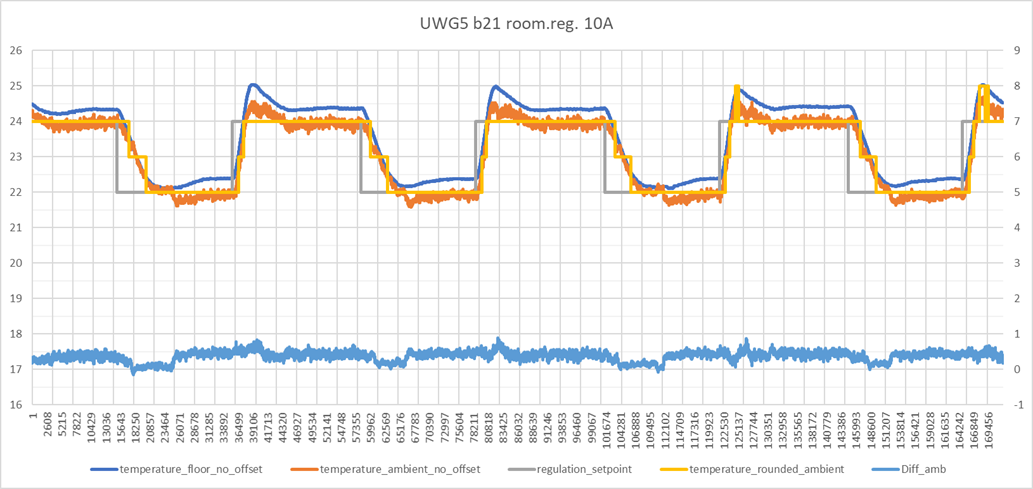
\includegraphics[width=1\linewidth]{figures/uwg5_test2.png}
    \caption{Test case 1 with 10 Amperes and 17\degree C outside}
    \label{fig:uwg5_testcase2}
\end{figure}
\begin{figure}[htbp]
    \centering
    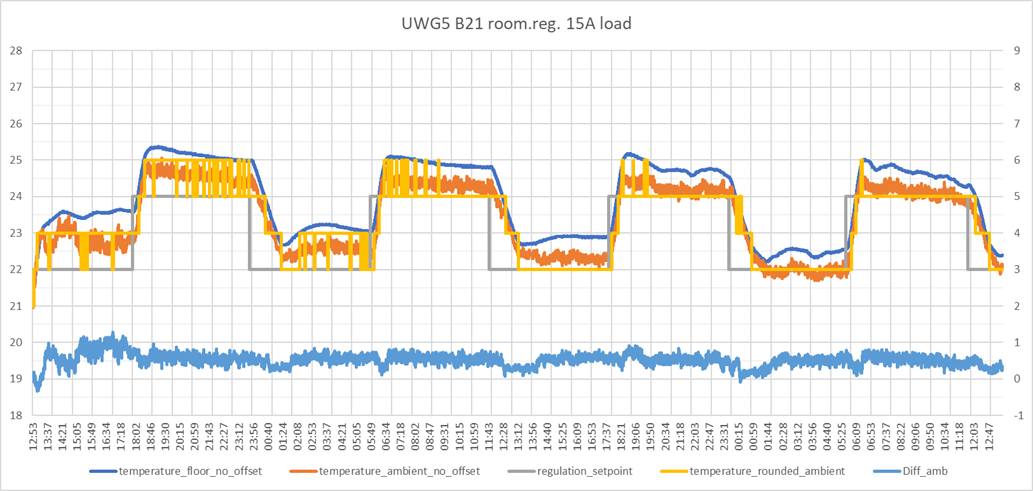
\includegraphics[width=1\linewidth]{figures/uwg5_test3.png}
    \caption{Test case 2 with 15 Amperes and 17\degree C outside}
    \label{fig:uwg5_testcase3}
\end{figure}
\begin{figure}[htbp]
    \centering
    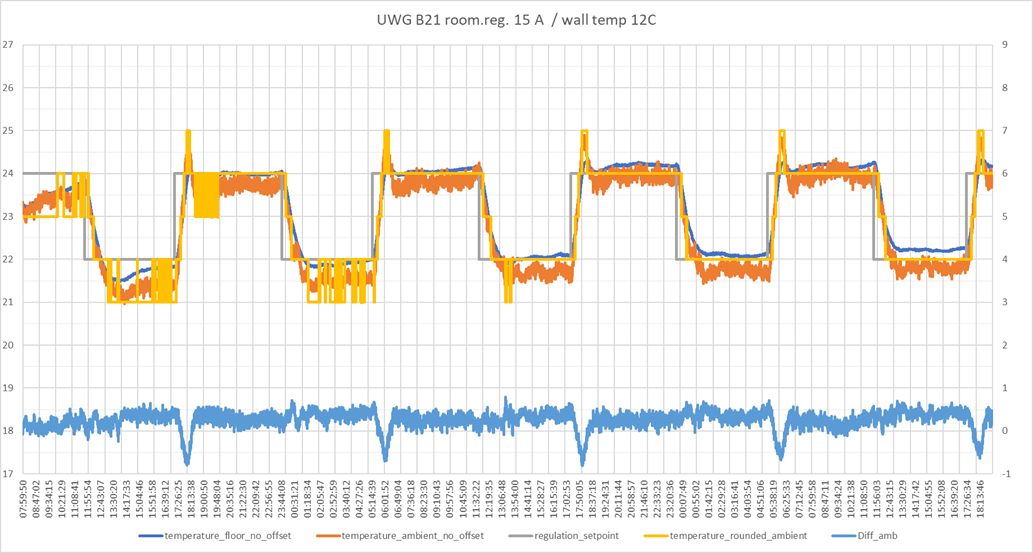
\includegraphics[width=1\linewidth]{figures/uwg5_test4.png}
    \caption{Test case 3 with 15 Amperes and 12\degree C outside}
    \label{fig:uwg5_testcase4}
\end{figure}

\nomenclature[N]{$n_r$}{Number of relay switches, when a relay turns on and off, it is one switch of two clicks.}

\end{document}